%%%%%%%%%%%%%%%%%%%%%%%%%%%%%%%%%%%%%%%%%%%%%%%%%%%%%%%%%%%%%%%%%%%%%%%%%%%%%%%%%%%%%%%%%%%%%%%%%%%%%%%%%%%%%%%%%%%%%%%%%%%%%%%%%%%%%%%%%%%%%%%%%%%%%%%%%%%
% This is just an example/guide for you to refer to when submitting manuscripts to Frontiers, it is not mandatory to use Frontiers .cls files nor frontiers.tex  %
% This will only generate the Manuscript, the final article will be typeset by Frontiers after acceptance.   
%                                              %
%                                                                                                                                                         %
% When submitting your files, remember to upload this *tex file, the pdf generated with it, the *bib file (if bibliography is not within the *tex) and all the figures.
%%%%%%%%%%%%%%%%%%%%%%%%%%%%%%%%%%%%%%%%%%%%%%%%%%%%%%%%%%%%%%%%%%%%%%%%%%%%%%%%%%%%%%%%%%%%%%%%%%%%%%%%%%%%%%%%%%%%%%%%%%%%%%%%%%%%%%%%%%%%%%%%%%%%%%%%%%%

%%% Version 3.3 Generated 2016/11/10 %%%
%%% You will need to have the following packages installed: datetime, fmtcount, etoolbox, fcprefix, which are normally inlcuded in WinEdt. %%%
%%% In http://www.ctan.org/ you can find the packages and how to install them, if necessary. %%%
%%%  NB logo1.jpg is required in the path in order to correctly compile front page header %%%

\documentclass[utf8]{frontiersSCNS} % for Science, Engineering and Humanities and Social Sciences articles
%\documentclass[utf8]{frontiersHLTH} % for Health articles
%\documentclass[utf8]{frontiersFPHY} % for Physics and Applied Mathematics and Statistics articles

%\setcitestyle{square} % for Physics and Applied Mathematics and Statistics articles
\usepackage{url,hyperref,lineno,microtype,subcaption,soul}
\usepackage[onehalfspacing]{setspace}
\usepackage{acronym}
\acrodef{EEG}{electroencephalography}
\acrodef{ICA}{independent component analysis}
\acrodef{PCA}{principal component analysis}
\acrodef{rCA}{Correlated component analysis}
\acrodef{ERP}{event-related potential}
\acrodef{BCI}{Brain-computer interface}
\acrodef{SSEP}{steady state evoked potential}

\linenumbers


% Leave a blank line between paragraphs instead of using \\


\def\keyFont{\fontsize{8}{11}\helveticabold }
\def\firstAuthorLast{Sample {et~al.}} %use et al only if is more than 1 author
\def\Authors{Avital Sternin\,$^{1,*}$, Bobby Stojanoski\,$^{1}$, Adrian M. Owen\,$^{1}$ and Jessica A. Grahn\,$^{1}$ }
% Affiliations should be keyed to the author's name with superscript numbers and be listed as follows: Laboratory, Institute, Department, Organization, City, State abbreviation (USA, Canada, Australia), and Country (without detailed address information such as city zip codes or street names).
% If one of the authors has a change of address, list the new address below the correspondence details using a superscript symbol and use the same symbol to indicate the author in the author list.
\def\Address{$^{1}$ Brain and Mind Institute, Department of Psychology, University of Western Ontario, London, ON, Canada}
% The Corresponding Author should be marked with an asterisk
% Provide the exact contact address (this time including street name and city zip code) and email of the corresponding author
\def\corrAuthor{Avital Sternin}
\def\corrEmail{avital.sternin@uwo.ca}




\begin{document}
\onecolumn
\firstpage{1}

\title[Running Title]{Article Title} 

\author[\firstAuthorLast ]{\Authors} %This field will be automatically populated
\address{} %This field will be automatically populated
\correspondance{} %This field will be automatically populated

\extraAuth{}% If there are more than 1 corresponding author, comment this line and uncomment the next one.
%\extraAuth{corresponding Author2 \\ Laboratory X2, Institute X2, Department X2, Organization X2, Street X2, City X2 , State XX2 (only USA, Canada and Australia), Zip Code2, X2 Country X2, email2@uni2.edu}


\maketitle


\begin{abstract}

%%% Leave the Abstract empty if your article does not require one, please see the Summary Table for full details.
abstract words here
\tiny
 \keyFont{ \section{Keywords:} keyword, keyword, keyword, keyword, keyword, keyword, keyword, keyword} %All article types: you may provide up to 8 keywords; at least 5 are mandatory.
\end{abstract}

\section{Introduction}
The search for a method to convey our intentions without employing speech or actions has preoccupied researchers for decades.
In particular, patients who are fully conscious and awake, yet are unable to respond behaviourally due to brain damage \citep{Owen2006,Monti2010,Cruse2011}, expose the necessity for alternate forms of communication. 
Over the past 30 years, \ac{EEG} studies have provided significant insights into how ``neural responsivity'' might be used to drive motor-independent communication.
\acp{BCI} using \ac{EEG} rely on large scale changes in brain states like P300 evoked potentials \citep{Farwell1988,Mugler2010,Tanaka2005}, sensorimotor rhythms \citep{Blankertz2011, Pfurtscheller2001}, or signals such as visual evoked potentials \citep{miranda2011brain, Wang2006} for gross control of an external device.
Generally, these interfaces allow users to make a binary choice. 

A binary choice system has its limitations however, and creating a \ac{BCI} that allows patients to communicate using more than two options is needed.
Creating such a system requires inducing more than two distinct brain states that can be consistently differentiated.
Results from previous studies show that perceived rhythms (a serious of tones arranged in a particular pattern) create distinct patterns in an EEG signal that can be identified \citep{stober2014}.
Distinct rhythmic patterns could be used to control a \ac{BCI} but they must be actively induced by the patient. 
An active way to induce such rhythms is for the patient to imagine the rhythmic patterns. 
Imagining a rhythmic pattern may induce the same changes in brain state as listening to a rhythm allowing us to classify these changes.
However, imagining a series of tones in a rhythmic pattern may be difficult for a patient to do, so a stimulus that is more salient and easier to imagine is necessary.
Speech is inherently rhythmic and may be easier to imagine than tones. 
Therefore, imagination of rhythmic speech phrases could be used to induce distinct rhythmic patterns in the brain.
There is some precedent as both heard \citep{Formisano2008} and imagined \citep{Deng2010} rhythmic patterns of vowel sounds have been classified from EEG signals. 

Deciphering the raw \ac{EEG} data is a difficult task because the electrical signals recorded at the scalp include a mixture of neural activity and noise (e.g., cardiac artifacts, eye blinks, movement, and electrical environmental noise), significant covariation between electrodes adds redundancy to the data, and some electrode sites do not capture the dynamic activity of the brain as well as others. 
Methods such as \ac{PCA} and \ac{ICA} provide a means to recover meaningful information from within the data. 
Recently, a new technique has emerged.
\ac{rCA} is computationally similar to \ac{PCA} in that it computes an eigenvalue decomposition of covariance data, but where \ac{rCA} differs is in the source of the covariance; \ac{rCA} operates on the pooled within-subject cross covariance

\begin{equation}
R_w=\frac{1}{N}\sum_{k=1}^{N} R_{kk},
\end{equation}
and pooled between-subjects cross covariance
\begin{equation}
R_b=\frac{1}{N(N-1)}\sum_{k=1}^{N}\sum_{l=1,l\neq{k}}^{N} R_{kl}
\end{equation}
where
\begin{equation}
R_{kl}=\sum_{t}(x_{k}(t)-\bar{x}_{k})(x_{l}(t)-\bar{x}_{l})^{T}
\end{equation}
calculates the cross-covariance between participant $k$ and participant $l$ across all electrodes $x$ at time $t$. The eigenvectors $w_{i}$ of the cross-covariance matrix $R_{w}^{-1}R_{b}$, with the largest eigenvalues $\lambda_{i}$ calculated as $(R_{w}^{-1}R_{b})w_{i} = \lambda_{i}w_{i}$ are the components that maximize Pearson's correlation between subjects in the data. Like the component ranking of PCA based on explained variance, components found using \ac{rCA} are rank-ordered by the magnitude of their correlation. 
The time courses and accompanying spatial weights of these correlated components represent patterns of evoked neural activity which are maximally correlated across all participants. 

In this experiment, participants listened to and imagined short, repeated rhythms composed of tones or words to induce different rhythmic brain states.
We investigated whether we could decode a user's \ac{EEG} signal to determine which rhythm or speech phrase they were listening to or imagining.
We used correlated components analysis to investigate our data.
The components represent information that similarly tracks the stimulus across two recordings and may carry information that is specific to each imagined rhythm that allow us to classify which rhythm or speech pattern a participant is listening to or imagining. 

\section{Materials and Methods}
\subsection{Participants}
Twelve participants (4 male), aged 20-27, with normal hearing and no history of brain injury took part in this study. Nine participants had formal musical training (1-15 years), and six of the participants played instruments regularly at the time of data collection.
\subsection{Stimuli}
Eight different stimuli were used during this experiment: four rhythmic patterns and four rhythm-matched speech phrases (see \autoref{fig:stimuli}). 
The speech phrases were chosen to be clinically relevant (That hurts; I'm hungry; No, I don't; Yes, I'd like that).
The audio was recorded in the lab along with a metronome to ensure exact timing.
The audiofiles of the stimuli can be found in the supplemental materials. 
Each trial consisted of a perception and an imagination component and was preceded by four metronome clicks to cue the participant to the tempo of the rhythm and speech patterns (120 bpm/2 Hz). 
Following the metronome cue, one of the eight stimuli would begin to play while the metronome continued.
After 12 seconds, the stimulus stopped playing, the metronome continued, and participants were asked to imagine the stimulus for another 12 seconds. 
Rhythmic pattern stimuli were played in a random order during the first half of the experiment and speech phrase stimuli were played in a random order during the second half. 
Rhythm always preceded speech so that participants would not inadvertently imagine the speech patterns during the rhythm block.
Each stimulus was heard and imagined 12 times throughout the experiment.
\subsection{Equipment and Procedure}
During the experiment, participants were seated in an audiometric room (Eckel model CL-13) and the \ac{EEG} data were collected using a BioSemi Active-Two system with 64+2 EEG channels. 
Horizontal and vertical EOG channels were used to record eye movements. \ac{EEG} was sampled at 512 Hz. 
A Cedrus StimTracker was used to ensure minimal delay ($<$0.05 ms) between the presentation of the stimulus to the participant and the marking of stimulus onset in the data. 
The experiment was programmed and presented using PsychToolbox run in MATLAB 2014a. A computer monitor displayed the instructions and speakers played the stimuli at a comfortable volume for each participant. 
While listening and imagining, participants were presented with a fixation cross and asked to keep their gaze steady.
The volume of the stimuli was kept constant across participants.
\subsection{Analysis}
\subsubsection{Preprocessing}
\ac{EEG} pre-processing was done using EEGLab. 
Data were filtered between 0.5 Hz and 30 Hz, downsampled to 256 Hz, epoched to remove break-periods, and submitted to an \ac{ICA} analysis.
\ac{ICA} components corresponding to artefacts (eyeblinks, heart rate, etc.) were manually removed.
The remaining components were used to reconstruct the EEG data.
\subsubsection{Correlational Component Analysis (rCA)}
Pooled within and between-subjects covariances were computed separately for each of the eight stimuli conditions. 
Only the top component extracted from each condition (i.e., the spatial weights and time course which maximized Pearson's correlation in the group-aggregate data) was considered for further analysis here. 
Although components $i = 2 ... n$ undoubtedly encompass various aspects of the experience of listening and imagining, the top component reflects some neural processes that are most common across subjects and provides an optimal starting point to evaluate the utility of ISC as a means of capturing the different brain states during each condition. 
\subsubsection{Inter-subject correlation and classification}
To assess the reliability of the correlated component at the single-subject level, time-resolved ISCs were computed by back projecting the component vectors $w_{i}$ into the original subject data to derive a component time course for each participant. 
We did this for each stimulus condition. 
With this per-subject time course, a measure of ISC encompassing the entire duration of the clip was computed first to quantify the magnitude of the correlation between each individual participant and the group and establish a distribution of synchronization in healthy controls; this is similar to the ISC analysis computed by \cite{Naci2015}. 
To generate the distribution of ISCs, Pearson's correlations were calculated between all possible pairs of subjects using a sliding window technique. A sliding window of $0.5$ seconds with a 60\% overlap was used to generate a correlation coefficient between pairs at two-second intervals over the course of the audio. 
\hl{This yielded 152 correlation coefficients for each of the 105 comparisons.}
The correlations computed for all subject pairs were then standardized using a Fisher's Z transformation and averaged at each time point to produce a mean ISC time course for each of the stimuli conditions. 
The time courses of the components were then used to classify which stimulus a participant was listening to or imagining. 
\subsubsection{Statistical analyses}
Non-parametric permutation statistics were used to test the significance of the group-averaged component time course for each of the stimuli conditions. 
Null distributions of correlation coefficients were created by iteratively phase-shifting the computed component time course for each participant and computing mean of the pairwise correlations with the rest of the group for each of the 152 time windows \citep{theiler1992testing}. 
We did this 1000 times to generate a null distribution of potential correlation values. The upper 5\% of each null distribution was used as the significance threshold for each time point. 
Significance levels were adjusted for multiple comparisons using a false discovery rate (FDR) correction. 
The number of significant two-second time windows was then compared between the intact and scrambled conditions using a Chi-square test of proportion with an alpha level set to .05. 

\section{Results}
rCA results 

classification results

\section{Discussion}
Using \ac{rCA} we were able to classify our stimuli at a statistically significant level within type (speech or rhythm) and modality (perception or imagination) indicating that both perceived and imagined stimuli are able to induce changes in the EEG signal that can be differentiated. 
Using the time courses of correlated components to classify our stimuli technique indicates that the differences across stimuli are maintained across people. 
In other words, the brains of participants are doing similar things as they listen to or imagine the same rhythmic and speech stimuli.

When we trained and tested our classifier on the same type of stimuli (rhythm/speech) within the same modality (perception/imagery) the classifier was able to differentiate the stimuli at 100\% accuracy.
When we trained and tested our classifier across modality (e.g. trained on speech perception and tested on speech imagination) our classifier was differentiating pairs of stimuli at chance levels. 
This lack of classification accuracy indicates that the time courses of the correlated components in perception and imagination are too similar for the classifier to be able to tell them apart.
This supports previous work showing similarities between the brain's perception and imagination processes (CITE).

When we trained and tested our classifier across stimulus type (e.g. trained on rhythm perception and tested on speech perception or vice versa) the results were varied.
Some pairs of stimuli could be differentiated at above chance levels.
The pattern of sounds in the rhythm and speech stimuli were the same but were presented either using tones in the rhythm condition or using words in the speech condition.
The similarities of this pattern of sounds between the two types of stimuli may be reflected in the time courses of the correlated components and the cross-type classification is being driven by the inherent rhythmic patterns of the stimuli. 
Although not all stimulus pairs could be classified at statistically significant levels the fact that some could be classified is an indication that perhaps the stimuli themselves are not suited to this type of classification and that this result is not due to a deficit in analysis technique.

mixed

scrambled 

We can classify within a modality (perception/imagination) - synchrony can be driven by internally generated sources.
Compare rhythm/speech.
What are the characteristics of the stim that are classified well/poorly? Not time signature. 

Takeaway: rCA is a simple, yet powerful tool that can be used to classify imagined brain states. The rhythmicity of speech stimuli can be used to produce differentiable brain states introducing a new technique that could be used to drive a \ac{BCI}.

%\paragraph{Level 4}
%\subparagraph{Level 5}

\section*{Conflict of Interest Statement}
The authors declare that the research was conducted in the absence of any commercial or financial relationships that could be construed as a potential conflict of interest.

\section*{Author Contributions}
AS contributed to the conception and design of the study, data collection, and preliminary analyses. BS contributed to analyses. All authors contributed to manuscript writing and revision and have read and approved the submitted version. 
\section*{Funding}
AS: NSERC (CGSM) 
BS:
JAG:
AMO:
Details of all funding sources should be provided, including grant numbers if applicable.

\section*{Acknowledgments}
Sebastian Stober for assistance in the study design.
This is a short text to acknowledge the contributions of specific colleagues, institutions, or agencies that aided the efforts of the authors.

\section*{Supplemental Data}
 \href{http://home.frontiersin.org/about/author-guidelines#SupplementaryMaterial}{Supplementary Material} should be uploaded separately on submission, if there are Supplementary Figures, please include the caption in the same file as the figure. LaTeX Supplementary Material templates can be found in the Frontiers LaTeX folder 


\bibliographystyle{frontiersinSCNS_ENG_HUMS} % for Science, Engineering and Humanities and Social Sciences articles, for Humanities and Social Sciences articles please include page numbers in the in-text citations
%\bibliographystyle{frontiersinHLTH&FPHY} % for Health, Physics and Mathematics articles
\bibliography{speechbib}

%%% Make sure to upload the bib file along with the tex file and PDF
%%% Please see the test.bib file for some examples of references

\section*{Figure captions}

%%% Please be aware that for original research articles we only permit a combined number of 15 figures and tables, one figure with multiple subfigures will count as only one figure.
%%% Use this if adding the figures directly in the mansucript, if so, please remember to also upload the files when submitting your article
%%% There is no need for adding the file termination, as long as you indicate where the file is saved. In the examples below the files (logo1.jpg and logos.jpg) are in the Frontiers LaTeX folder
%%% If using *.tif files convert them to .jpg or .png
%%%  NB logo1.jpg is required in the path in order to correctly compile front page header %%%

\begin{figure}[h!]
\begin{center}
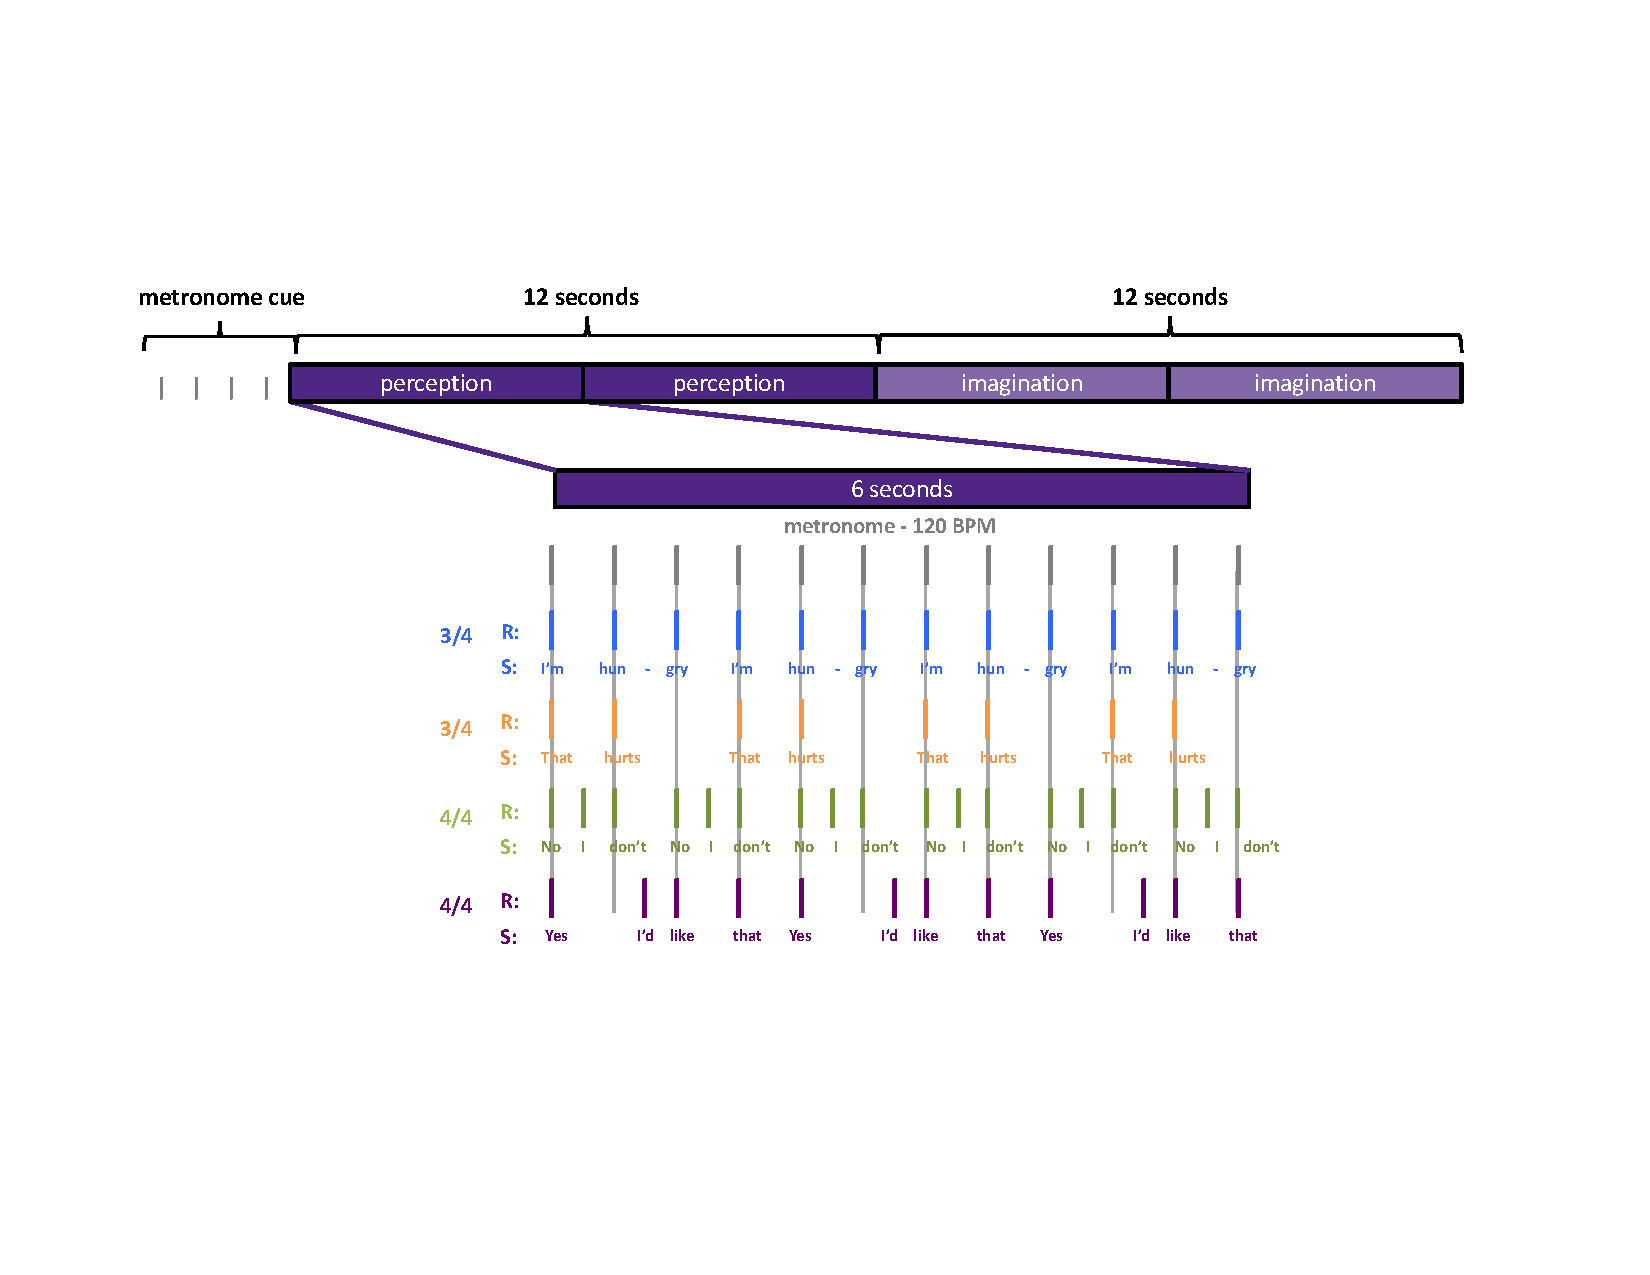
\includegraphics[width=17cm]{Figures/SpeechFigure}
\end{center}
\caption{A single trial involved 2 seconds of a metronome cue, 12 seconds of perception, and 12 seconds of imagination. The metronome continued throughout the perception and imagination periods. The 8 stimuli (4 rhythm and 4 speech) are pictured. Half of the stimuli were written in musical 3/4 time and half were written in musical 4/4 time. The coloured bars in the rhythm conditions indicate when a tone was heard, the words below indicate the corresponding speech phrase.}
\label{fig:stimuli}
\end{figure}

\end{document}
